\documentclass{article}
\usepackage{graphicx} % Required for inserting images
\usepackage{fancyhdr} % Header
\usepackage{lastpage}
\usepackage[a4paper, total={6in, 8in}]{geometry}
\usepackage{float} % Floating position
\usepackage{hyperref} % Links
\usepackage{amsmath} % Math
\usepackage{amssymb} % Math
\usepackage{bbold} % Math (for indicatrice function)
\usepackage{listings} % Import code in appendix
\usepackage{pdfpages} % Include PDF
\usepackage{tikz} % Graph
\usetikzlibrary{bayesnet}
\usetikzlibrary{positioning}

\graphicspath{{images/}}

\newcommand{\authorFst}{Tristan Perrot}
\newcommand{\emailFst}{\href{mailto:tristanp@kth.se}{tristanp@kth.se}}

\pagestyle{fancy}
\fancyhf{} % clear all header and footer fields
\lhead{Assignment 1B \\ DD2434 - Machine Learning, Advanced Course}
\rhead{\authorFst}
\cfoot{\thepage \  / \pageref{LastPage}}
\setlength{\headheight}{23pt}
\setlength{\footskip}{70pt}

\title{DD2434 - Machine Learning, Advanced Course \\ Assignment 1B}
\author{\authorFst \\ \emailFst}
\date{November 2023}

\begin{document}

\maketitle

\begin{center}
  \includegraphics[scale=0.5]{KTH_logo_RGB_bla.png}
\end{center}

\thispagestyle{empty}

\newpage
\tableofcontents
\newpage

\section{CAVI for Earth quakes}

\subsection{Question 1.1}

\begin{figure}[H]
  \centering
  \begin{tikzpicture}

% Custom style for nodes without a border
    \tikzstyle{plain} = [draw=none, fill=none]

    % Define nodes
    \node[latent] (z) {$Z_n$};
    \node[plain, above=of z] (pi) {$\pi$};
    \node[latent, below left=of z] (s) {$S_n$};
    \node[latent, below right=of z] (x) {$X_n$};
    \node[latent, below=of s] (lambda) {$\lambda$};
    \node[latent, below=of x] (mu) {$\mu$};
    \node[plain, right=of x] (tau) {$\tau$};
    \node[plain, below=of lambda] (alpha) {$\alpha$};
    \node[plain, left=of alpha] (beta) {$\beta$};
    \node[plain, below=of mu] (nu) {$\nu$};
    \node[plain, left=of nu] (rho) {$\rho$};

    % Connect nodes
    \edge {pi} {z};
    \edge {z} {x, s};
    \edge {lambda} {s};
    \edge {mu} {x};
    \edge {tau} {x};
    \edge {alpha, beta} {lambda};
    \edge {nu, rho} {mu};

    % Plates
    \plate [inner sep=0.3cm] {plate1} {(z)(s)(x)} {$N$}; % Adjusted position and size
    \plate [inner xsep=0.3cm] {plate2} {(mu)(lambda)} {$K$}; % Adjusted position and size


\end{tikzpicture}

  \label{fig:fig1}
  \caption{Directed Graphical Model for the Earthquake problem}
\end{figure}

\subsection{Question 1.2}

Let us take the Alternative 1 in 2D. Here, we know these distributions:
\begin{itemize}
  \item $p(Z_n|\pi) = Categorical(\pi)$
  \item $p(S_n|Z_n = k, \lambda_k) = Poisson(\lambda_k)$
  \item $p(X_n|Z_n = k, \mu_k, \tau) = Normal(\mu_k, \tau \cdot I)$
  \item $p(\mu_k|\nu,\rho) = Normal(\nu, \rho \cdot I)$
  \item $p(\lambda_k|\alpha, \beta) = Gamma(\alpha, \beta)$
\end{itemize}
Where, $\rho$ and $\tau$ define precision and not standard variation. Then we have:
\begin{equation}
  \begin{split}
    \log p(X,S,Z,\lambda,\mu|\pi,\tau,\alpha,\beta,\nu,\rho) & = \log p(X|S,Z,\lambda,\mu,\pi,\tau,\alpha,\beta,\nu,\rho)                 \\
                                                             & \qquad\qquad + \log p(S,Z,\lambda,\mu|\pi,\alpha,\beta,\nu,\rho)           \\
                                                             & = \log p(X|Z,\mu,\tau) + \log p(S|Z,\lambda,\mu,\pi,\alpha,\beta,\nu,\rho) \\
                                                             & \qquad\qquad + \log p(Z,\lambda,\mu|\pi\alpha,\beta,\nu,\rho)              \\
                                                             & = \log p(X|Z,\mu,\tau) + \log p(S|Z,\lambda) + \log p(Z|\pi)               \\
                                                             & \qquad\qquad + \log p(\lambda,\mu|\alpha,\beta,\nu,\rho)                   \\
    \log p(X,S,Z,\lambda,\mu|\pi,\tau,\alpha,\beta,\nu,\rho) & = \log p(X|Z,\mu,\tau) + \log p(S|Z,\lambda) + \log p(Z|\pi)               \\
                                                             & \qquad\qquad + \log p(\mu|\nu,\rho) + \log p(\lambda|\alpha,\beta)         \\
  \end{split}
\end{equation}

Where:
\begin{equation}
  \begin{split}
    \log p(X|Z,\mu,\tau)         & = \sum_{n=1}^{N}\sum_{k=1}^{K}\log p(X_n|Z_n = k, \mu_k, \tau) \\
    \log p(S|Z,\lambda)          & = \sum_{n=1}^{N}\sum_{k=1}^{K}\log p(S_n|Z_n = k, \lambda_k)   \\
    \log p(Z|\pi)                & = \sum_{n=1}^{N}\log p(Z_n|\pi)                                \\
    \log p(\mu|\nu,\rho)         & = \sum_{k=1}^{K}\log p(\mu_k|\nu,\rho)                         \\
    \log p(\lambda|\alpha,\beta) & = \sum_{k=1}^{K}\log p(\lambda_k|\alpha,\beta)                 \\
  \end{split}
\end{equation}

\subsection{Question 1.3}

Here, the mean field approximation is not an approximation but an equality because $Z, \mu, \lambda$ are independent. Therefore we have:
\begin{equation}
  \begin{split}
    \log q^*(Z_n) & \overset{+}{=} \mathbb{E}_{\mu,\lambda}[\log p(X_n,S_n,Z_n,\lambda,\mu|\pi,\tau,\alpha,\beta,\nu,\rho)]                                                                          \\
                  & \overset{+}{=} \mathbb{E}_{\mu,\lambda}[\log p(X_n|Z_n,\mu,\tau) + \log p(S_n|Z_n,\lambda) + \log p(Z_n|\pi)]                                                                    \\
                  & = \mathbb{E}_{\mu}\left[\sum_{k=1}^{K}\mathbb{1}_{\{Z_n = k\}}\left(\log \left(\frac{\tau}{2\pi}\right) -\frac{\tau}{2}\left((x_n - \mu_k)^T(x_n - \mu_k)\right)\right)\right]   \\
                  & \qquad\qquad + \mathbb{E}_{\lambda}\left[\sum_{k=1}^{K}\mathbb{1}_{\{Z_n = k\}}\left(\log(\pi_k) -\lambda_k + S_n\log(\lambda_k) - \log(S_n!)\right)\right]                      \\
                  & \overset{+}{=} \sum_{k=1}^{K}\mathbb{1}_{\{Z_n = k\}}\left(\log \left(\frac{\tau}{2\pi}\right) - \frac{\tau}{2}\mathbb{E}_{\mu}\left[(x_n - \mu_k)^T(x_n - \mu_k)\right] \right. \\
                  & \qquad\qquad \left. + \log(\pi_k) + \mathbb{E}_{\lambda}\left[-\lambda_k + S_n\log(\lambda_k)\right] - \log(S_n!)\right)
  \end{split}
\end{equation}
Now, if we take the entire expression that is multiplied by $\mathbb{1}_{\{Z_n = k\}}$ and we call it $u_{n,k}$, we have:
\begin{equation}
  q^*(Z_n) \propto \prod_{k=1}^{K}u_{n,k}^{\mathbb{1}_{\{Z_n = k\}}}
\end{equation}
And if we normalize by taking $r_{n,k} = \frac{u_{n,k}}{\sum_{i=1}^{K}u_{n,i}}$ we get:
\begin{equation}
  q^*(Z_n) = \prod_{k=1}^{K}r_{n,k}^{\mathbb{1}_{\{Z_n = k\}}}
\end{equation}
Wich means that $q^*(Z_n)$ is a categorical distribution with parameters $r_{n,k}$. There for we have the expectation of $Z_n$ easily because $\mathbb{E}[z_{n,k}] = r_{n,k}$ where $z_{n,k} = \mathbb{1}_{\{S_n = k\}}$. Note that $r_{n,k}$ depends of the expected value of $\mu_k$, $\mu_k^2$, $\lambda_k$ and $\log \lambda_k$. We will be able to compute these expected values by finding $q^*(\mu_k)$ and $q^*(\lambda_k)$.

\noindent Let us compute $q^*(\mu_k)$:
\begin{equation}
  \begin{split}
    \log q^*(\mu_k) & \overset{+}{=} \mathbb{E}_{Z,\lambda}[\log p(X,S,Z = k,\lambda_k,\mu_k|\pi,\tau,\alpha,\beta,\nu,\rho)]                                                                                                  \\
                    & \overset{+}{=} \mathbb{E}_{Z,\lambda}[\log p(X|Z = k,\mu_k,\tau) + \log p(\mu_k|\nu,\rho)]                                                                                                               \\
                    & = \mathbb{E}_{Z,\lambda}\left[\sum_{n=1}^{N}\mathbb{1}_{\{Z_n = k\}}\left(\log \left(\frac{\tau}{2\pi}\right) -\frac{\tau}{2}\left((x_n - \mu_k)^T(x_n - \mu_k)\right)\right)\right]                     \\
                    & \qquad\qquad + \log \left(\frac{\rho}{2\pi}\right) - \frac{\rho}{2}\left((\mu_k - \nu)^T(\mu_k - \nu)\right)                                                                                             \\
                    & \overset{+}{=} \sum_{n=1}^{N}r_{n,k}\left(\log \left(\frac{\tau}{2\pi}\right) - \frac{\tau}{2}\left((x_n - \mu_k)^T(x_n - \mu_k)\right)\right) - \frac{\rho}{2}\left((\mu_k - \nu)^T(\mu_k - \nu)\right) \\
                    & \overset{+}{=} \sum_{n=1}^{N}r_{n,k}\left(-\frac{\tau}{2}\left((x_n - \mu_k)^T(x_n - \mu_k)\right)\right) - \frac{\rho}{2}\left((\mu_k - \nu)^T(\mu_k - \nu)\right)                                      \\
                    & \overset{+}{=} - \frac{\tau\sum_{n=1}^{N}r_{n,k}}{2}\left(-2\mu_{k,0}x_{n,0} -2\mu_{k,1}x_{n,1} +\mu_{k,0}^2 +\mu_{k,1}^2\right)                                                                         \\
                    & \qquad\qquad - \frac{\rho}{2}\left(-2\mu_{k,0}\nu_0 -2\mu_{k,1}\nu_1 +\mu_{k,0}^2 +\mu_{k,1}^2\right)
  \end{split}
\end{equation}
We define $S = \frac{\rho}{\tau\sum_{n=1}^{N}r_{n,k}}$. Then we have:
\begin{equation}
  \begin{split}
    \log q^*(\mu_k) & \overset{+}{=} -\frac{\tau\sum_{n=1}^{N}r_{n,k}}{2}\left[(S+N)\mu_{k,0}^2 + (S+N)\mu_{k,1}^2 \right.                                                                                      \\
                    & \qquad\qquad \left. -2\mu_{k,0}(S\nu_0 + \sum_{n=1}^{N}x_{n,0}) -2\mu_{k,1}(S\nu_1 + \sum_{n=1}^{N}x_{n,1})\right]                                                                        \\
                    & \overset{+}{=} -\frac{\tau\sum_{n=1}^{N}r_{n,k}}{2(S+N)}\left[\left(\mu_k - \frac{S\nu + \sum_{n=1}^{N}x_n}{S+N}\right)^T\left(\mu_k - \frac{S\nu + \sum_{n=1}^{N}x_n}{S+N}\right)\right]
  \end{split}
\end{equation}
Therefore, we have $q^*(\mu_k) = Normal\left(\mu^*, \rho^* \cdot I\right)$. And we can compute the expected value of $\mu_k$ and $\mu_k^2$ easily.

\begin{equation}
  \begin{split}
    \mu^*  & = \frac{S\nu + \sum_{n=1}^{N}x_n}{S+N}   = \frac{\rho\nu + \tau\sum_{n=1}^{N}r_{n,k}x_n}{\rho + N\tau\sum_{n=1}^{N}r_{n,k}} \\
    \rho^* & = \frac{\tau\sum_{n=1}^{N}r_{n,k}}{S+N} = \frac{(\tau\sum_{n=1}^{N}r_{n,k})^2}{\rho + N\tau\sum_{n=1}^{N}r_{n,k}}
  \end{split}
\end{equation}
And therefore:
\begin{equation}
  \begin{split}
    \mathbb{E}[\mu_k]   & = \mu^*                            \\
    \mathbb{E}[\mu_k^2] & = \frac{1}{\rho^*} + \mu^{*T}\mu^*
  \end{split}
\end{equation}

\noindent Let us compute $q^*(\lambda_k)$:
\begin{equation}
  \begin{split}
    \log q^*(\lambda_k) & \overset{+}{=} \mathbb{E}_{Z,\mu}[\log p(X,S,Z = k,\lambda_k,\mu_k|\pi,\tau,\alpha,\beta,\nu,\rho)]                             \\
                        & \overset{+}{=} \mathbb{E}_{Z,\mu}[\log p(S|Z = k,\lambda_k) + \log p(\lambda_k|\alpha,\beta)]                                   \\
                        & = \mathbb{E}_{Z}\left[\sum_{n=1}^{N}\mathbb{1}_{\{Z_n = k\}}\left(-\lambda_k + S_n\log(\lambda_k) - \log(S_n!)\right)\right]    \\
                        & \qquad\qquad + \log \left(\frac{\beta^\alpha}{\Gamma(\alpha)}\right) + (\alpha - 1)\log(\lambda_k) - \beta\lambda_k             \\
                        & \overset{+}{=} \sum_{n=1}^{N}r_{n,k}\left(-\lambda_k + S_n\log(\lambda_k)\right) + (\alpha - 1)\log(\lambda_k) - \beta\lambda_k \\
                        & = \left(\alpha + \sum_{n=1}^{N}S_n r_{n,k} - 1\right)\log(\lambda_k) - \left(\beta + \sum_{n=1}^{N}r_{n,k}\right)\lambda_k
  \end{split}
\end{equation}
Therefore, we have $q^*(\lambda_k) = Gamma\left(\alpha + \sum_{n=1}^{N}S_n r_{n,k}, \beta + \sum_{n=1}^{N}r_{n,k}\right)$. And we can compute the expected value of $\lambda_k$ and $\log \lambda_k$ easily.
\begin{equation}
  \begin{split}
    \mathbb{E}[\lambda_k]      & = \frac{\alpha + \sum_{n=1}^{N}S_n r_{n,k}}{\beta + \sum_{n=1}^{N}r_{n,k}}       \\
    \mathbb{E}[\log \lambda_k] & = \psi(\alpha + \sum_{n=1}^{N}S_n r_{n,k}) - \log(\beta + \sum_{n=1}^{N}r_{n,k})
  \end{split}
\end{equation}

\section{VAE image generation}
\subsection*{Question 5.1 (in the notebook)}
Our objective function is ELBO: $E_{q(z|x)}\big[\log \frac{p(x,z)}{q(z|x)}\big]$ \\
We will show that ELBO can be rewritten as $E_{q(z|x)}\big(\log p(x|z)\big) - D_{KL} \big( q(z|x) \lvert \rvert  p(z)\big)$
We have:
\begin{align*}
  E_{q(z|x)}\big[\log \frac{p(x,z)}{q(z|x)}\big] & = E_{q(z|x)}\big[\log p(x,z) - \log q(z|x)\big]                                                     \\
                                                 & = E_{q(z|x)}\big[\log p(x|z) + \log p(z) - \log q(z|x)\big]                                         \\
                                                 & = E_{q(z|x)}\big[\log p(x|z)\big] + E_{q(z|x)}\big[\log p(z)\big] - E_{q(z|x)}\big[\log q(z|x)\big] \\
                                                 & = E_{q(z|x)}\big[\log p(x|z)\big] - E_{q(z|x)}\big[\log \frac{q(z|x)}{p(z)}\big]                    \\
                                                 & = E_{q(z|x)}\big[\log p(x|z)\big] - D_{KL} \big( q(z|x) \lvert \rvert  p(z)\big)
\end{align*}

\subsection*{Question 5.2 (in the notebook)}
Consider the second term: $- D_{KL} \big( q(z|x) \lvert \rvert  p(z)\big)$

\textit{\textbf{Question :} Kullback–Leibler divergence can be computed using the closed-form analytic expression when both the variational and the prior distributions are Gaussian. Write down this KL divergence in terms of the parameters of the prior and the variational distributions. Your solution should consider a generic case where the latent space is K-dimensional.}

We have:
\begin{align*}
  D_{KL} \left(q(z|x) \lvert\rvert p(z)\right) & = \int q(z|x) \log \frac{q(z|x)}{p(z)} \,dz
\end{align*}

And we also have:
\begin{equation}
  \begin{split}
    q(z|x) & = \mathcal{N}(z|\mu(x), \sigma(x)) = \prod_{i=1}^{K}\left(\frac{1}{\sigma_i\sqrt{2\pi}} \exp\left(-\frac{(z_i - \mu_i)^2}{2\sigma^2}\right)\right)                                    \\
    p(z)   & = \mathcal{N}(z|0, I) = \left(\frac{1}{\sqrt{2\pi}}\right)^K \exp\left(-\frac{1}{2}z^Tz\right) = \prod_{i=1}^{K}\left(\frac{1}{\sqrt{2\pi}}\right) \exp\left(-\frac{1}{2}z_i^2\right)
  \end{split}
\end{equation}

Therefore:
\begin{equation}
  \begin{split}
    D_{KL} \left(q(z|x) \lvert\rvert p(z)\right) & = \int q(z|x) \log \frac{q(z|x)}{p(z)} \,dz                                                                                                                                                                                         \\
                                                 & = \int q(z|x) \log \frac{\prod_{i=1}^{K} \left(2\pi\sigma_i^2\right)^{-\frac{1}{2}} \exp\left(-\frac{(z_i - \mu_i)^2}{2\sigma_i^2}\right)}{\prod_{i=1}^{K} \left(2\pi\right)^{-\frac{1}{2}} \exp\left(-\frac{z_i^2}{2}\right)} \,dz \\
                                                 & = \int q(z|x)  \left(\sum_{i=1}^{K} -\log (\sigma_i) - \frac{(z_i - \mu_i)^2}{2\sigma_i^2} + \frac{z_i^2}{2}\right) \,dz                                                                                                            \\
                                                 & = \mathbb{E}_{q(z|x)}\left[\sum_{i=1}^{K} -\log (\sigma_i) - \frac{(z_i - \mu_i)^2}{2\sigma_i^2} + \frac{z_i^2}{2}\right]                                                                                                           \\
                                                 & = \sum_{i=1}^{K} -\log(\sigma_i) - \frac{\mathbb{E}_{q(z|x)}\left[(z_i - \mu_i)^2\right]}{2\sigma_i^2} + \frac{\mathbb{E}_{q(z|x)}\left[z_i^2\right]}{2}                                                                            \\
                                                 & = \sum_{i=1}^{K} -\log(\sigma_i) - \frac{\sigma_i^2}{2\sigma_i^2} + \frac{\mathbb{E}_{q(z|x)}[z_i^2]}{2}                                                                                                                            \\
                                                 & = \sum_{i=1}^{K} -\log(\sigma_i) - \frac{1}{2} + \frac{\sigma_i^2 + \mu_i^2}{2}                                                                                                                                                     \\
    D_{KL} \left(q(z|x) \lvert\rvert p(z)\right) & = \frac{1}{2} \sum_{i=1}^{K} \left(\sigma_i^2 + \mu_i^2 - \log(\sigma_i^2) - 1\right)
  \end{split}
\end{equation}

The rest of tht implementation could be find in the appendix \ref{appendix:1.2}.

\section{Reparameterization and the score function}
\subsection{Question 3.4}

According to the \href{https://arxiv.org/abs/1703.09194}{Sticking the Landing} paper, we can do the reparameterization by sampling z from a parametric distribution $q_\phi(z)$ and by sampling $\epsilon$ from a fixed distribution $p(\epsilon)$ and applying a deterministic transformation $t(\epsilon, \phi) = z$
Therefore, we have for the total derivative of the ELBO term:
\begin{equation}
  \begin{split}
    \hat{\nabla}_{\text{TD}}(\epsilon,\phi) & = \nabla_\phi[\log p(z|x) + \log p(x) - \log q_\phi (z|x)]                                              \\
                                            & = \nabla_z[\log p(z|x) - \log q_\phi(z|x)] \nabla_\phi z - \nabla_\phi \log q_\phi(z|x)                 \\
                                            & = \nabla_z[\log p(z|x) - \log q_\phi(z|x)] \nabla_\phi t(\epsilon, \phi) - \nabla_\phi \log q_\phi(z|x) \\
  \end{split}
\end{equation}
Where the left term is the score function.

\subsection{Question 3.5}
Now, we will show that the expectation of the score function is zero.
\begin{equation}
  \begin{split}
    \mathbb{E}_{q_\phi(z|x)}\left[\nabla_\phi \log q_\phi(z|x)\right] & = \int q_\phi(z|x) \nabla_\phi \log q_\phi(z|x) \,dz \\
                                                                      & = \int \nabla_\phi q_\phi(z|x) \,dz                  \\
                                                                      & = \nabla_\phi \int q_\phi(z|x) \,dz                  \\
                                                                      & = \nabla_\phi 1                                      \\
                                                                      & = 0
  \end{split}
\end{equation}

\subsection{Question 3.6}
In the \href{https://arxiv.org/abs/1703.09194}{Sticking the Landing} paper, the author handle this score function by removing it and it results in an unbiased gradient estimator with variance that approaches zero as the approximate posterior approaches the exact posterior.

\subsection{Question 3.7}
For particular cases, the score function may actually decrease the variance. The name of the concept that describes how the score function acts in this situation is \textbf{control variate}.

\section{Reparameterization of common distributions}
\subsection{Question 4.8 - Exponential distribution}
The exponential distribution is defined as:
\begin{equation}
  p(x|\lambda) = \lambda \exp(-\lambda x)
\end{equation}
Here, we can use the inverse of the cumulative distribution function to sample from this distribution. The cumulative distribution function is:
\begin{equation}
  F(x) = 1 - \exp(-\lambda x)
\end{equation}
Therefore, the inverse of the cumulative distribution function is:
\begin{equation}
  F^{-1}(x) = -\frac{1}{\lambda} \log(1 - x)
\end{equation}
And as stated in the \href{https://arxiv.org/abs/1703.09194}{Sticking the Landing} paper, we can sample $u$ from the uniform distribution $U(0,1)$ and apply the inverse of the cumulative distribution function to get a sample from the exponential distribution. Therefore, we have:
\begin{equation}
  z = -\frac{1}{\lambda} \log(1 - u)
\end{equation}
The implementation of the reparameterization of the exponential distribution can be found in the appendix \ref{appendix:1.4}.

\subsection{Question 4.9 - Categorical distribution}
\subsubsection{Approximation by the Gumbel-Sofmax distribution}
Using the \href{https://arxiv.org/abs/1611.01144}{Categorical Reparameterization with Gumbel-Softmax} paper, we can describe how to reparameterize the categorical distribution.
We have $z$ categorical variable with class probabilities $\pi_1, \dots, \pi_z$. We can sample $z$ from the categorical distribution by sampling $z$ from the Gumbel-Max distribution. The Gumbel-Max distribution is defined as:
\begin{equation}
  G_i = -\log(-\log(u_i))
\end{equation}
Where $u_i$ are sampled from the uniform distribution $U(0,1)$. And then sample $y_i$ with Softmax:
\begin{equation}
  y_i = \frac{\exp((\log(\pi_i) + G_i)/\tau)}{\sum_{j=1}^{z}\exp((\log(\pi_j) + G_j)/\tau)}
\end{equation}
Where $\tau$ is the temperature parameter.

\subsubsection{Using the argmax function}
For evaluation purposes, we can use the argmax function to get the most probable class. Therefore, we have:
\begin{equation}
  z = \text{one hot} \left(\arg\max_i [G_i + \log \pi_i]\right)
\end{equation}
The implementation of the reparameterization of the categorical distribution can be found in the appendix \ref{appendix:1.4}.

\newpage
\appendix

\section{Appendix}
\subsection{VAE image generation}\label{appendix:1.2}
\includepdf[pages=-]{code/1B-VAE.pdf}

\subsection{Reparameterization of common distributions}\label{appendix:1.4}
\includepdf[pages=-]{code/1B-Reparameterization.pdf}


\end{document}